\documentclass[10pt]{seminar} 

\renewcommand{\baselinestretch}{1}

\usepackage{amsmath}

\renewcommand{\printlandscape}{\special{landscape}}

\usepackage{ulem}



\input{seminar.bug}

%\usepackage{fancybox}

\usepackage{epsfig}

%\usepackage{times}


\usepackage{amssymb}

\usepackage{amscd}

\usepackage{graphics}

\usepackage{pstricks}

%\usepackage{chicago}

%\usepackage{fullpage}

\slideframe{none}

\begin{document}

\newtheorem{proposition}{Proposition}

\newtheorem{definition}{Definition}

\newtheorem{corollary}{Corollary}

\newtheorem{theorem}{Theorem}

\newtheorem{lemma}{Lemma}

\def\argmax{\mathop{\rm argmax}\limits}  


%\slideframe{Oval}

\sffamily 


\begin{slide}
\begin{center}

Matrix algebra
 \end{center}
 
 \newslide
 \small 
 
 A \textit{vector} is a list of numbers: $\mathbf{a}=(2, 4, 5, 1)$ 
 
 $$\mathbf{a}= \begin{bmatrix}
  2\\4\\5\\1
\end{bmatrix}$$

\ \\The $i$th component of $\mathbf{a}$ is denoted $a_i$ (above, $a_3=5$)

\ \\A vector with $n$ components is an $n-$vector

\ \\The set of all $n-$vectors with real numbers as components is $\mathbb{R}^n$

\newslide

Vector arithmetic is very similar to ordinary arithmetic

\ \\Certain operations impose a restriction on the number of components the vectors can have (e.g. $\mathbf{a}+\mathbf{b}$ requires $\mathbf{a}$ and $\mathbf{b}$ to be the same length)

$$
\hbox{Addition: }
\begin{bmatrix}
a_1\\a_2\\ ... \\a_n
\end{bmatrix}
+
\begin{bmatrix}
b_1\\b_2\\ ... \\b_n
\end{bmatrix}
=
\begin{bmatrix}
a_1+b_1\\a_2+b_2\\ ... \\a_n+b_n
\end{bmatrix}
$$

$$
\hbox{Scalar multiplication:  \hspace{.2in}}
\lambda \begin{bmatrix}
a_1\\a_2\\ ... \\a_n
\end{bmatrix}
=
\begin{bmatrix}
\lambda a_1\\\lambda a_2\\ ... \\ \lambda a_n
\end{bmatrix}
$$


\newslide

Vector arithmetic geometrically

\begin{center}
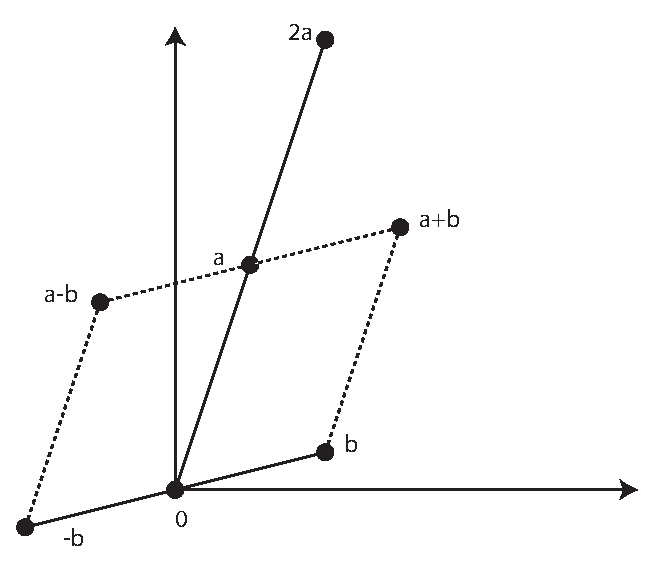
\epsfig{file=arith.eps, scale=.6}
\end{center}

\newslide

Linear dependence

\ \\A linear combination of vectors $\mathbf{a, b, c, ...} $ is a new vector of the form
$$\alpha \mathbf{a}+ \beta \mathbf{b}+\gamma \mathbf{c}+...$$ where $\alpha, \beta, \gamma$ are scalars (elements of $\mathbb{R}$) and can potentially equal zero

\ \\A set of $k$ vectors $\mathbf{a^1, a^2, ..., a^k}$ is \textit{linearly dependent} if it is possible to express one of the vectors as a linear combination of the others

\ \\The set is \textit{linearly independent} if it's \textit{not} possible to express one as a linear combination of the others


\newslide

Example: 

$$
\mathbf{a}=
\begin{bmatrix}
2 \\ 3
\end{bmatrix},
\mathbf{b}=
\begin{bmatrix}
1 \\ 1
\end{bmatrix},
\mathbf{c}=
\begin{bmatrix}
3 \\ 2
\end{bmatrix}
$$
These vectors are linearly dependent because $\mathbf{b}={1\over 5}(\mathbf{a}+\mathbf{c})$

\ \\Criterion for linear dependence:  $\mathbf{a^1, a^2, ..., a^k}$ are \textit{linearly dependent} if there exist scalars $\alpha_1, \alpha_2, ..., \alpha_k$ that are \textit{not all equal to zero} such that $$\alpha_1 \mathbf{a}^1+\alpha_2 \mathbf{a}^2+...+\alpha_n \mathbf{a}^n=0$$

\ \\(In the above example, $\alpha_a=\alpha_c={1\over 5}$ and $\alpha_b=-1$)

\newslide
How to test for linear dependence

\ \\We can solve for the scalars explicitly:

$$
\mathbf{a}=
\begin{bmatrix}
2 \\ 3
\end{bmatrix},
\mathbf{b}=
\begin{bmatrix}
1 \\ 1
\end{bmatrix},
\mathbf{c}=
\begin{bmatrix}
3 \\ 2
\end{bmatrix}
$$

$$\begin{array}{rcl}
2\alpha_a+\alpha_b+3\alpha_c&=&0 \\
3\alpha_a+\alpha_b+2\alpha_c&=&0 
 \\
-2\alpha_a-3\alpha_c &=& \alpha_b\\
 \\
 3\alpha_a-2\alpha_a-3\alpha_c+2\alpha_c&=&0
\end{array}
$$

$$\alpha_a=\alpha_c \hbox{ and } \alpha_b=-5\alpha_a$$
(The vectors are linearly dependent)

\newslide
Example of linear independence
$$
\mathbf{a}=
\begin{bmatrix}
1 \\ 3 \\ 1
\end{bmatrix},
\mathbf{b}=
\begin{bmatrix}
1 \\ 1 \\1
\end{bmatrix},
\mathbf{c}=
\begin{bmatrix}
3 \\ 2 \\1
\end{bmatrix}
$$

$$\begin{array}{rcl}
\alpha_a+\alpha_b+3\alpha_c&=&0 \\
3\alpha_a+\alpha_b+2\alpha_c&=&0 \\
\alpha_a+\alpha_b+\alpha_c&=&0\\
\\
-\alpha_a-3\alpha_c&=&\alpha_b \\
3\alpha_a -\alpha_a-3\alpha_c +2\alpha_c&=&0\\
2\alpha_a&=&\alpha_c\\
\alpha_a-7\alpha_a+2\alpha_a&=&0\\
\alpha_a=\alpha_b=\alpha_c&=&0
\end{array}
$$

\newslide
Matrices

\ \\A matrix is a rectangular array of numbers; a matrix with $m$ rows and $n$ columns is called an $m\times n$ matrix

\ \\The entry in the $i$th row and $j$th  column of a matrix is the $(i, j)$ entry of the matrix

$$
\mathbf{A}=\begin{bmatrix}
2 & 3&  5&  2&  1\\
3 &16 & 1  &4  &5\\
0 &6 &1 &10&8\\
\end{bmatrix}
$$

\ \\$\mathbf{A}$ is a $3\times 5$ matrix, with $a_{25}=5$, $a_{34}=10$, etc.

\newslide
Matrix arithmetic

\ \\Addition and scalar multiplication work the same as for vectors:

$$
\begin{bmatrix}
1&2&3\\
1&3&3\\
\end{bmatrix}
+
\begin{bmatrix}
10&12&2\\
10&0&30\\
\end{bmatrix}
=
\begin{bmatrix}
11&14&5\\
11&3&33\\
\end{bmatrix}$$

$$
5\begin{bmatrix}
1&2&3\\
1&3&3\\
\end{bmatrix}
=
\begin{bmatrix}
5&10&15\\
5&15&15\\
\end{bmatrix}
$$

\newslide
Matrix multiplication

\ \\Example: A $2\times 3$ matrix, $\mathbf{A}$, and a 3-vector $\mathbf{x}=(x_1, x_2, x_3)$
$$\mathbf{A}=
\begin{bmatrix}
 6 & 8& 7\\
 5& 1& 9
\end{bmatrix} \hbox{ and }
 \mathbf{x}=\begin{bmatrix}
 x_1\\
 x_2\\
 x_3
\end{bmatrix}
$$

$\mathbf{Ax}$ is the following 2-vector:

$$
\begin{bmatrix}
 6 & 8& 7\\
 5& 1& 9
\end{bmatrix}
\begin{bmatrix}
 x_1\\
 x_2\\
 x_3
\end{bmatrix}
=
\begin{bmatrix}
6x_1+8x_2+7x_3\\
5x_1+x_2+9x_3
\end{bmatrix}
$$

\newslide

$$
\begin{bmatrix}
 6 & 8& 7\\
 5& 1& 9
\end{bmatrix}
\begin{bmatrix}
 x_1\\
 x_2\\
 x_3
\end{bmatrix}
=
\begin{bmatrix}
6x_1+8x_2+7x_3\\
5x_1+x_2+9x_3
\end{bmatrix}
$$

Points to note
\begin{itemize}
\item The system of equations 
$$\begin{array}{rcl}
6x_1+8x_2+7x_3&=&b_1\\
5x_1+x_2+9x_3&=&b_2
\end{array}
$$ can be written as $\mathbf{Ax}=\mathbf{b}$, with $\mathbf{b}=(b_1, b_2)$
\item The $2\times 3$ matrix $\mathbf{A}$ turns a 3-vector into a 2-vector; we can think of $\mathbf{A}$ as a mapping from $\mathbb{R}^3$ into $\mathbb{R}^2$
\end{itemize}

\newslide

Matrix multiplication more generally

\ \\Let $\mathbf{A}$ be an $m\times n$ matrix and $\mathbf{B}$ be an $n\times s$ matrix; then $\mathbf{A}\mathbf{B}$ is an $m\times s$ matrix with entry $(i, j)$ equal to $$(i, j)=\sum_{k=1}^n a_{ik}b_{kj}$$


\ \\Each entry $(i, j)$ takes the sum of the product of each $i$th row entry in $\mathbf{A}$ with the $j$th column entry in $\mathbf{B}$

\ \\Example:

$$\mathbf{A}=\begin{bmatrix}
a_{11}& a_{12}\\
a_{21} & a_{22}
\end{bmatrix}, 
\mathbf{B}=\begin{bmatrix}
b_{11}& b_{12}\\
b_{21} & b_{22}
\end{bmatrix},
\mathbf{AB}=\begin{bmatrix}
a_{11}b_{11}+a_{12}b_{21}&a_{11}b_{12}+a_{12}b_{22}\\
a_{21}b_{11}+a_{22}b_{21}& a_{21}b_{12}+a_{22}b_{22}
\end{bmatrix} $$

\newslide

Bigger example:

$$
\mathbf{A}=\begin{bmatrix}
1& 5\\
2 & -3\\
4 & -8
\end{bmatrix}, 
\mathbf{B}=\begin{bmatrix}
2& -7 & 3& 0\\
1 & 0& 4& -5
\end{bmatrix}
$$
$$
\mathbf{AB}=\begin{bmatrix}
1 \times 2+5\times 1& 1\times -7+5\times 0 & 1\times 3+5\times 4 & 1\times 0+5\times -5\\
 2\times 2-3\times 1& 2\times -7-3\times 0& 2\times 3-3\times 4& 2\times 0-3\times -5\\
 4\times 2-8\times 1& 4\times -7-8\times 0& 4\times 3-8\times 4& 4\times 0-8\times -5\\
\end{bmatrix}
$$

$$
\mathbf{AB}=\begin{bmatrix}
7& -7& 23& -25\\
1& -14& -6&15\\
0&-28&-20& 40\\
\end{bmatrix}
$$

\newslide

Important facts about matrix multiplication

\begin{itemize}
\item We can multiply any two matrices $\mathbf{AB}$ when the number of columns in $\mathbf{A}$ equals the number of rows in $\mathbf{B}$

$$\underbrace{\mathbf{A}}_{n\times m}\underbrace{\mathbf{B}}_{m\times k}=\underbrace{\mathbf{C}}_{n\times k}$$
\item Matrix multiplication is NOT commutative

$$\mathbf{AB}\not=\mathbf{BA}$$
\begin{itemize}
\item First, both sides are only defined if $\mathbf{A}$ is $n\times m$ and $\mathbf{B}$ is $m\times n$
\item Even if $\mathbf{A}$ is $m\times m$ and $\mathbf{B}$ is $m\times m$ they may still not be the same
$$\mathbf{A}=
\begin{bmatrix}
0 & 1\\
1& 0
\end{bmatrix}
\mathbf{B}=
\begin{bmatrix}
0& 1\\
2& 0
\end{bmatrix}
$$
\end{itemize}

\end{itemize}

\newslide

The $n\times n$ identity matrix, $\mathbf{I}_n$

\ \\This is an $n\times n$ matrix whose $(i, j)$ entry is 1 if $i=j$ and $0$ otherwise

$$\mathbf{I}_3=
\begin{bmatrix}
 1 & 0& 0\\
 0 & 1& 0\\
 0& 0& 1
\end{bmatrix}$$

If $A$ is $n\times m$, then $$\mathbf{I}_n\mathbf{A}=\mathbf{A}$$ and $$\mathbf{A}\mathbf{I}_m=\mathbf{A}$$

\newslide
Echelon matrices

An echelon matrix has the following two properties:

\begin{itemize}
\item[1] There's at least one non-zero entry and rows with all zeros lie below rows that have at least one non-zero entry
\item[2] In each row after the first, the left-most non-zero entry lies to the right of the left-most non-zero entry in the preceding row


$$\begin{bmatrix}
\star &\cdot& \cdot& \cdot \\
 0 &\star &\cdot& \cdot\\
 0& 0& 0& \star \\
 0&0&0&0
\end{bmatrix}
$$
\item The first non-zero entry in each row $(\star)$ is the \textit{pivot}
\end{itemize}

\newslide
Gaussian elimination (creating echelon matrices to solve $\mathbf{Ax=B}$)

\ \\The following are the elementary operations we'll use:
\begin{itemize}
\item Exchanging two rows
\item Subtracting a multiple of one row from another

\end{itemize}

We will subtract multiples of one row (the pivot row) from each of the rows below it

\ \\We'll work with an augmented matrix

$$\begin{bmatrix}\mathbf{A}&|&\mathbf{b}\end{bmatrix}$$

\newslide

Suppose we want to solve  $\mathbf{Ax=B}$  for $\mathbf{x}$, with

$$\mathbf{A}=\begin{bmatrix}
2& -4& 1& -8\\
4& -8& 7& -6\\
-1& 2& 1& 7
\end{bmatrix}
\hbox{ and }
\mathbf{b}=
\begin{bmatrix}
-4\\
12\\
8
\end{bmatrix}$$

We start with augmented matrix

$$\begin{bmatrix}\mathbf{A}&\mathbf{b}\end{bmatrix}=
\begin{bmatrix}
2& -4& 1& -8&-4\\
4& -8& 7& -6&12\\
-1& 2& 1& 7&8
\end{bmatrix}
$$
\newslide
$$\begin{bmatrix}\mathbf{A}&\mathbf{b}\end{bmatrix}=
\begin{bmatrix}
2& -4& 1& -8&-4\\
4& -8& 7& -6&12\\
-1& 2& 1& 7&8
\end{bmatrix}
$$

Using the top row as a pivot we subtract multiples of pivot from each lower row (2 and $-{1\over 2}$, respectively):

$$\begin{bmatrix}
2& -4& 1& -8&-4\\
0& 0& 5& 10&20\\
0& 0& {3\over 2}& 3&6
\end{bmatrix}
$$

Using second row as a pivot we multiply it by ${3\over 10}$ and subtract from third:

$$\begin{bmatrix}
2& -4& 1& -8&-4\\
0& 0& 5& 10&20\\
0& 0& 0& 0&0
\end{bmatrix}
$$

\newslide
We're left with:
$$\begin{bmatrix}
2& -4& 1& -8&-4\\
0& 0& 5& 10&20\\
0& 0& 0& 0&0
\end{bmatrix}
$$

We have 2 equations and 4 unknowns; assign arbitrary values to $x_2=\lambda$ and $x_4=\mu$ (the entries without pivots)

$$\begin{array}{rcl}5x_3&=&20-10\mu\\
 x_3&=&4-2\mu
 \end{array}
$$ and 
$$\begin{array}{rcl}2x_1&=&4\lambda-(4-2\mu)+8\mu-4\\
x_1&=&-4+2\lambda+5\mu
\end{array}
$$ 
\newpage
Summarizing, we have

$$\begin{array}{rcl}
x_1&=&-4+2\lambda+5\mu\\
x_2&=&\lambda\\
 x_3&=&4-2\mu\\
 x_4&=&\mu
\end{array}$$

Which your book writes as

$$\mathbf{x}=
\begin{bmatrix}
-4\\0\\4\\0
\end{bmatrix}
+\lambda
\begin{bmatrix}
2\\1\\0\\0
\end{bmatrix}
+\mu
\begin{bmatrix}
5\\0\\-2\\1
\end{bmatrix}
$$

\newslide

Solve the system $\mathbf{Ax=b}$ where

$$\mathbf{A}=\begin{bmatrix}
2& 1& 4\\
2& 1& 1\\
4& 8& 7\\
4& 3& 9
\end{bmatrix}\hbox{ and }
\mathbf{b}=\begin{bmatrix}
5\\8\\5\\8
\end{bmatrix}
$$
%x1=5, x2=-1, x3=-1
\newslide

Matrix rank

\ \\The rank of a matrix $\mathbf{A}$ is the maximum number of linearly independent columns of $\mathbf{A}$; it is also the maximum number of linearly independent rows of $\mathbf{A}$

\ \\This is the dimension $(k)$ of the vector space $\mathbb{R}^k$ \textit{spanned} by its columns (or rows)

\ \\The \textit{span} of a set of a finite set of vectors $S$ is the set of all linear combinations of the elements of $S$; if this equals $\mathbb{R}^k$ then Span$(S)=\mathbb{R}^k$

\newslide

Rank and span

$$\mathbf{A}=\begin{bmatrix}
1&0&1\\
0&1&1\\
1&1&2
\end{bmatrix}$$

\ \\Columns 1 and 2 are linearly independent, but their sum equals Column 3; the rank of $\mathbf{A}=2$

These three vectors span $\mathbb{R}^2$ but not $\mathbb{R}^3$: Show that for any $(x_1, x_2)\in \mathbb{R}^2$, we can find a $\lambda_1, \lambda_2, \lambda_3$ such that $$\lambda_1(1, 0, 1)+\lambda_2(0, 1, 1)+\lambda_3(1, 1, 2)=(x_1, x_2, x_1+x_2)$$

They span $\mathbb{R}^2$ and the space of all vectors in $\mathbb{R}^3$ of form $(x_1, x_2, x_1+x_2)$

\ \\Show that for any $(x_1, x_2, x_3)\in \mathbb{R}^3$, we \textit{can't} find a $\lambda_1, \lambda_2, \lambda_3$ such that $$\lambda_1(1, 0, 1)+\lambda_2(0, 1, 1)+\lambda_3(1, 1, 2)=(x_1, x_2, x_3)$$

\newslide

Finding the rank of a matrix $\mathbf{A}$

\begin{itemize}
\item Reduce $\mathbf{A}$ to an echelon matrix $\mathbf{E}$ using Gaussian elimination
\item The number of non-zero rows of $\mathbf{E}$ is the rank of $\mathbf{A}$!
\end{itemize}

\vspace{.3in}
Properties of ranks

\begin{itemize}
\item The rank of an $n\times m$ matrix  $\mathbf{A}$ can't be greater than either $n$ or $m$: Rank($\mathbf{A}$)$\leq \min (n, m)$
\item A matrix has \textit{full rank} if its rank is the biggest it could be: Rank($\mathbf{A}$)$= \min (n, m)$
\item A square matrix is \textit{invertible} if and only if it has full rank
\end{itemize}

\newslide

Inverse Matrices

\ \\A square matrix $\mathbf{A}$ is \textit{singular} if the system of equations $\mathbf{Ax=0}$ has a non-zero solution for $\mathbf{x}$

\ \\$\mathbf{A}$ is \textit{non-singular} if the system of equations $\mathbf{Ax=0}$ has the unique solution $\mathbf{x=0}$

\ \\$\mathbf{A}$ is non-singular if and only if it has full rank

\ \\Why we care: If $n\times n$ matrix $\mathbf{A}$ is non-singular and $\mathbf{y}$ is any $n$-vector, then there is exactly one $n-$vector $\mathbf{x}$ that solves $$\mathbf{Ax=y}$$

\newslide
Square matrix $\mathbf{A}$ is invertible if there is a square matrix $\mathbf{A}^{-1}$ with the property that $$\mathbf{Ax=y} \hbox{ if and only if }\mathbf{x=A^{-1}y}$$

\ \\$\mathbf{A}^{-1}$ is the \textit{inverse} of $\mathbf{A}$

\ \\Obviously if we know $\mathbf{y}$ then we can solve $\mathbf{Ax=y}$ explicitly, just using Gaussian elimination

\ \\Inverses can be useful if we want to solve the above equation for \textit{any} $\mathbf{y}$

\newslide

How to invert a matrix

\ \\Take $$\begin{bmatrix}\mathbf{A I} \end{bmatrix}$$ and use Gauss-Jordan elimination to convert it into

\ \\$$\begin{bmatrix}\mathbf{I A^{-1}} \end{bmatrix}$$

\ \\Gauss-Jordan elimination is similar to Gaussian elimination, but turns matrix into a diagonal matrix, instead of just an echelon matrix

\newslide
Let's invert $$\mathbf{A}=\begin{bmatrix}
2&1&2\\
3&1&1\\
3&1&2
\end{bmatrix}$$


$$\hbox{Step 1: }\begin{bmatrix}
2&1&2& 1& 0& 0\\
3&1&1& 0& 1& 0\\
3&1&2& 0& 0&1
\end{bmatrix}$$

$$\hbox{Step 2: }\begin{bmatrix}
2&1&2& 1& 0& 0\\
0&-{1\over 2}&-2& -{3\over 2}&1 & 0\\
0&-{1\over 2}&-1& -{3\over 2}& 0&1
\end{bmatrix}$$

\newslide

$$\hbox{Step 2: }\begin{bmatrix}
2&1&2& 1& 0& 0\\
0&-{1\over 2}&-2& -{3\over 2}&1 & 0\\
0&-{1\over 2}&-1& -{3\over 2}& 0&1
\end{bmatrix}$$
Since we are creating a diagonal we want to get rid of the ``1" in (1, 2)

\vspace{.2in}
$$\hbox{Step 3: }\begin{bmatrix}
2&0&-2& -2& 2& 0\\
0&-{1\over 2}&-2& -{3\over 2}&1 & 0\\
0&0&1& 0& -1&1
\end{bmatrix}$$
This added 2 $\times$ Row 2 to Row 1 and subtracted Row 2 from Row 3

\newslide


$$\hbox{Step 3: }\begin{bmatrix}
2&0&-2& -2& 2& 0\\
0&-{1\over 2}&-2& -{3\over 2}&1 & 0\\
0&0&1& 0& -1&1
\end{bmatrix}$$
We get a diagonal matrix by adding 2 $\times $ Row 3 to Rows 1 \& 2  

$$\hbox{Step 4: }\begin{bmatrix}
2&0&0& -2& 0& 2\\
0&-{1\over 2}&0& -{3\over 2}&-1 & 2\\
0&0&1& 0& -1&1
\end{bmatrix}$$

We finish by normalizing
$$\hbox{Step 5: }\begin{bmatrix}
1&0&0& -1& 0& 1\\
0&1&0&3&2 & -4\\
0&0&1& 0& -1&1
\end{bmatrix}
\hbox{ and } \mathbf{A}^{-1}=
\begin{bmatrix}
 -1& 0& 1\\
3&2 & -4\\
 0& -1&1
\end{bmatrix}
$$

\newslide

Inverse facts
\begin{itemize}
\item $\mathbf{A}\mathbf{A}^{-1}=\mathbf{A}^{-1}\mathbf{A}=\mathbf{I}$
\item $(\mathbf{A}^{-1})^{-1}=\mathbf{A}$
\item If $\mathbf{A}$ and $\mathbf{B}$ are invertible so is $\mathbf{A}\mathbf{B}$ and $(\mathbf{AB})^{-1}=\mathbf{B}^{-1}\mathbf{A}^{-1}$
\item If $\mathbf{A}$ is $2 \times 2$ with $$\mathbf{A}=\begin{bmatrix}
a&b\\c&d
\end{bmatrix}$$  and $ad\not=bc$ then 

$$\mathbf{A}^{-1}={1\over{ad-bc}}\begin{bmatrix}
d&-b\\-c&a
\end{bmatrix}$$

(If $ad=bc$ then $\mathbf{A}$ isn't invertible)
\end{itemize}


 \end{slide}
 
 \end{document}








